\chapter{Experimental Setup}

This work evaluates the proposed algorithms for image and text data. This chapter describes the used datasets, the evaluation methods and the experimental setups.

\section{Datasets}
\label{sec:datasets}

\subsection{Never Ending Language Learner data}

The Never Ending Language Learner (NELL) is a learning agent that reads the web, extracts data and verfies beliefs \cite{Mitchell:2015:NL:2886521.2886641}\cite{Mitchell:2018:NL:3210350.3191513}. NELL for example knows that "Pittsburgh" is located in "Pennsylvania". These beliefs represent different noun-phrases such as "Pittsburgh" and "Pennsylvania". The noun-phrases belong to certain categories. "Pittsburgh" is a "City" and "Pennsylvania" is a "State". These subcategories both belong to the main category "Geopolitical Location". While there are already different subcategories, the goal for a hierarchical clustering algorithm here is to extract new useful subcategories.

The used dataset, extracted web-information by NELL, contains 32 different main categories, such as "Animal", "Location" or "Person". Each of these consists of up to 250 different entities that belong to different subcategories. Examplary entites for the category "Animal" are "Otter", "Squirrel" or "Wolf". 

This thesis shows in chapter \ref{sec:results} the learned subcategories.

\subsection{MNIST handwritten digits}

The MNIST handwritten digit database contains images of the handwritten digits from zero to nine \cite{lecun-mnisthandwrittendigit-2010}. Samples of these images are shown in figure \ref{fig:mnist} Its training set contains a total of 60,000 images, where each image is represented as a 784-dimensional vector corresponding to a greyscale image with 28x28 pixels.

\begin{figure}[h]
    \centering
    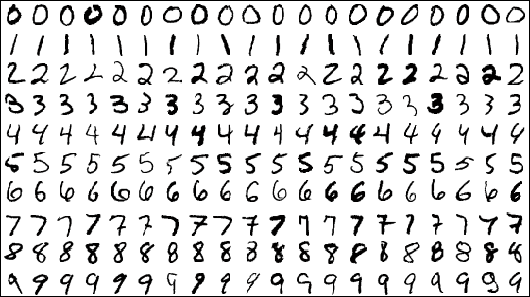
\includegraphics[width=0.7\textwidth]{images/mnist}
    \caption{The MNIST handwritten digits database contains 60,000 greyscale images of handwritten digits ranging from zero to nine. These samples show ten randomly drawn samples for each label represented as a 28x28 pixel image \cite{lecun-mnisthandwrittendigit-2010}.}
    \label{fig:mnist}
\end{figure}

The goal of clustering MNIST images is to find an unsupervised learning method that can distinguish between greyscale images. In addition, we can define various clustering tasks where we pick a subsample of the ten labels and then try to transfer the results to other subsamples. For example, we first cluster images labeled as zero, one, two, three or four and later apply the knowledge the learned gained for clustering images labeled as five, six, seven, eight or nine. Theses types of experiments allow high-level transfer learning if we define several different clustering tasks, e.g. for five different labels there are $10 \choose 5$ $= 252$ different combinations of labels.

Another obsevation that results from hierarchical clustering is the similarity of different labels, i.e. which labels are likely to get clustered together.

\subsection{CIFAR-10}

Another image dataset this thesis uses for evaluation is the CIFAR-10 dataset that contains 60,000 RGB images of ten different categories \cite{Krizhevsky2009LearningML}. Each image consists of 32x32 pixels and is thus represented as a 3072-dimensional vector (32x32x3). The categories and ten random images from each are shown in figure \ref{fig:cifar10}.

\begin{figure}[h]
    \centering
    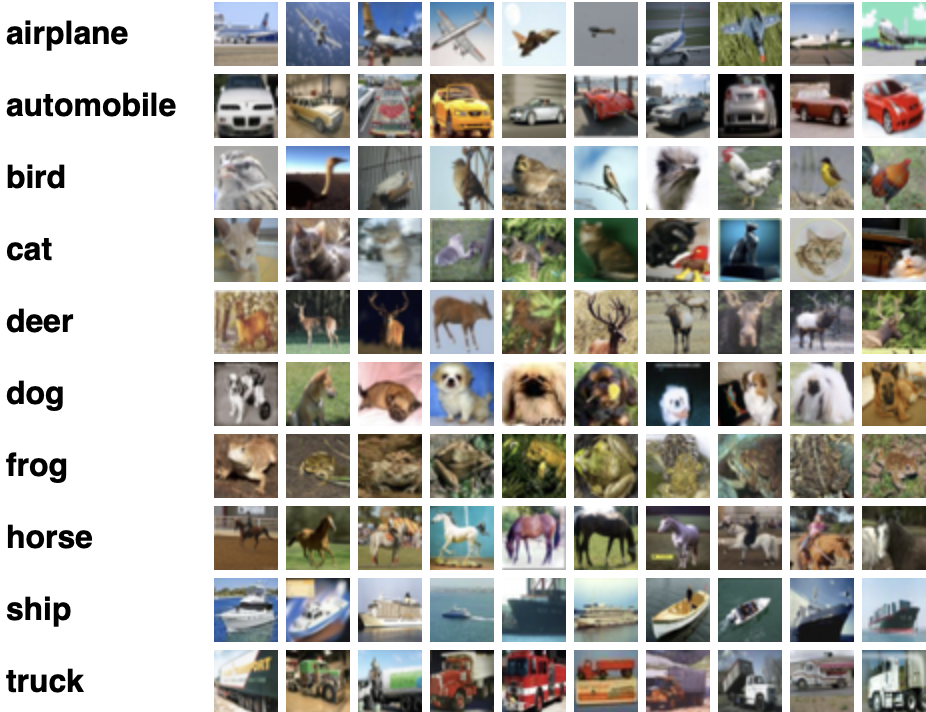
\includegraphics[width=0.7\textwidth]{images/cifar10}
    \caption{The CIFAR-10  database contains 60,000 RGB images of the ten shown different classes. These samples show ten randomly drawn samples for each label represented as a 32x32 pixel image \cite{Krizhevsky2009LearningML}.}
    \label{fig:cifar10}
\end{figure}

As the amount of images and the amount of classes is equal to the ones in the MNIST database, we can also try similar experiments. The main difference is that the images consist of RGB pixels instead of greyscale values.

\subsection{CIFAR-100}

The CIFAR-100 dataset contains similar images, but instead of 6,000 images each for 10 classes, it consists of 600 images each for 100 classes. The classes are divided into 20 superclasses each containing five subclasses. Examples of superclasses and corresponding subclasses are shown in table \ref{table:cifar100data}. 

\begin{table}[h]
    \centering
    \begin{tabular}{|l|l|}
    \hline
    superclass      & subclasses                                  \\ \hline
    aquatic mammals & beaver, dolphin, otter, seal, whale         \\
    fish            & aquarium fish, flatfish, ray, shark, trout  \\
    flowers         & orchids, poppies, roses, sunflowers, tulips \\
    people          & baby, boy, girl, man, woman                 \\ 
    reptiles        & crocodile, dinosaur, lizard, snake, turtle  \\ \hline               
    \end{tabular}
    \caption{The CIFAR-100 dataset contains 20 different superclasses, each with five different subclasses leading to 100 classes overall. The images are represented in the same way as in the CIFAR-10 dataset, i.e. by a 3072-dimensional vector \cite{Krizhevsky2009LearningML}.}
    \label{table:cifar100data}
\end{table}

Having superclasses and subclasses allows clustering between different subclasses within a superclass and also between different superclasses. This allows more experiments than for the CIFAR10 data.

\subsection{Omniglot}

The omniglot dataset contains 1623 handwritten characters from 50 different alphabets, where each character is represented by 20 different images. Each image is grayscale and represented by 105x105 pixels \cite{Lake1332}. Figure \ref{fig:omniglotcharacters} shows characters of the more well-known Latin, Greek and Hebrew alphabets that are part of the dataset.

\begin{figure}[h]
\centering
\begin{minipage}{.3\textwidth}
  \centering
  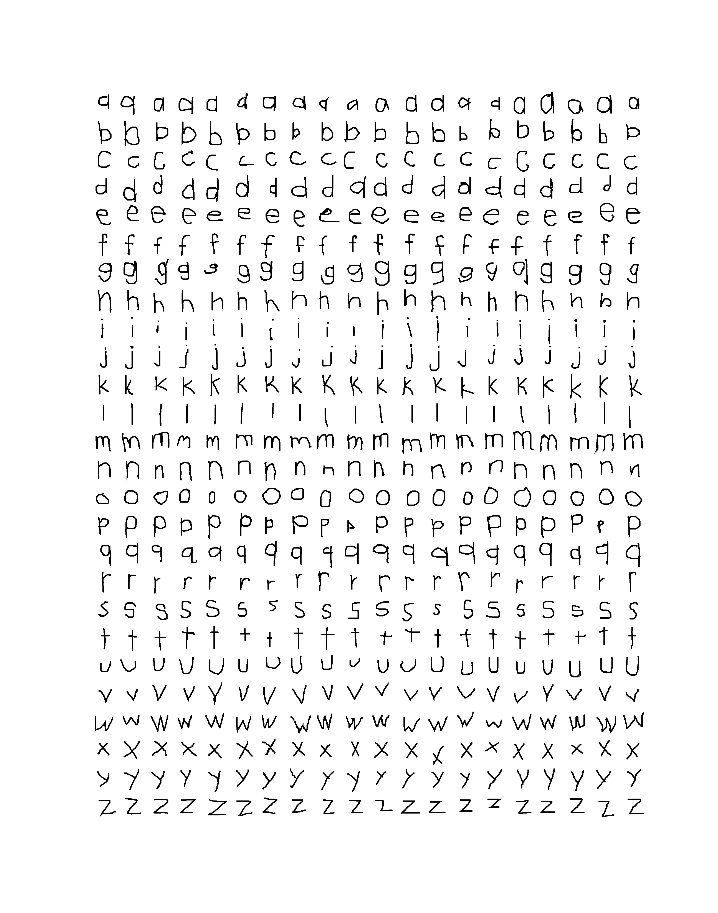
\includegraphics[width=\linewidth]{images/latin}
\end{minipage}
\begin{minipage}{.3\textwidth}
  \centering
  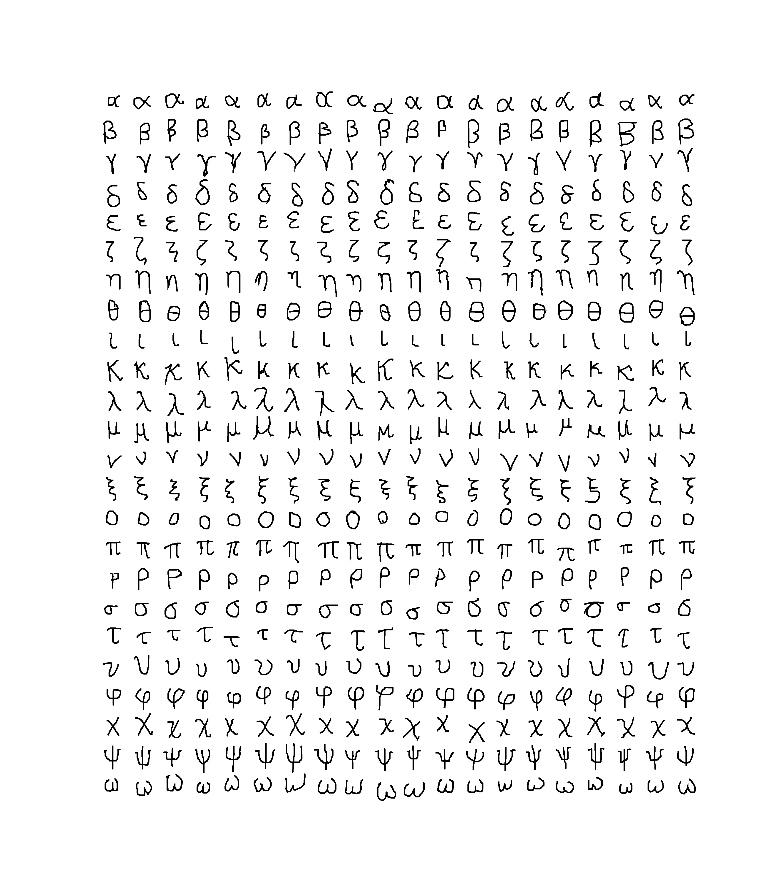
\includegraphics[width=\linewidth]{images/greek}
\end{minipage}
\begin{minipage}{.3\textwidth}
  \centering
  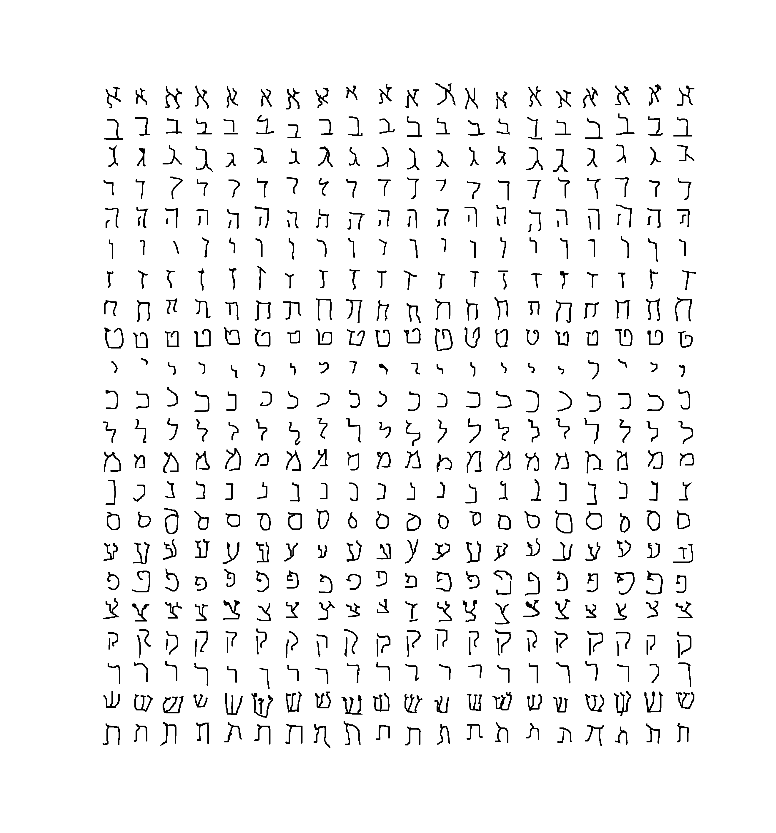
\includegraphics[width=\linewidth]{images/hebrew}
\end{minipage}
\caption{The omniglot dataset contains handwritten characters of different alphabets, such as Latin, Greek and Hebrew \cite{Lake1332}.}
\label{fig:omniglotcharacters}
\end{figure}

\section{Cost functions}

In order to evaluate the quality of a clustering, we need some kind of cost function that compares the generated clustering $C_1,...,C_k$ with the target clustering $C_1^*, ..., C_k^*$. One method to compare them is the majority distance as shown in equation \ref{eq:majoritydistance} where $n$ ist the number of sampled points.

\begin{equation}
    \begin{aligned}
        cost_{majority}(C_{1:k}, C_{1:k}^*) = \frac{1}{n} \sum\limits_{i=1}^{k} (\|C_i\| - \max\limits_j \|C_i \cap C_j^*\|)
    \end{aligned}
    \label{eq:majoritydistance}
\end{equation}

This cost function is motivated by finding corresponding clusters with the lowest distance, i.e. each generated cluster gets matched with the optimal target cluster. However two generated clusters can be matched with the same target cluster. This motivates the hamming distance as shown in figure \ref{eq:hammingdistance}.

\begin{equation}
    \begin{aligned}
        cost_{hamming}(C_{1:k}, C_{1:k}^*) = \max\limits_{\sigma} \frac{1}{n} \sum\limits_{i=1}^{k} (\|C_i\| - \max\limits_{\sigma, j} \|C_i \cap C_j^*\|)
    \end{aligned}
    \label{eq:hammingdistance}
\end{equation}

However, the hamming distance consists of an assignment problem to find the optimal matching $\sigma$ between the generated clusters and the target clusters. Table \ref{table:matching} shows how such a matching can look like.

\begin{table}[h]
    \centering
    \begin{tabular}{|l | l l l l l|}
    \hline
    j\textbackslash i & 1 & 2 & 3 & 4 & 5\\ \hline
    1 & 20 & \cellcolor{blue!25}15 & 30 & 50 & 40\\
    2 & 80 & 10 & \cellcolor{blue!25}15 & 20 & 30\\
    3 & \cellcolor{blue!25}20 & 30 & 50 & 80 & 60\\
    4 & 30 & 50 & 40 & \cellcolor{blue!25}20 & 10\\
    5 & 20 & 30 & 40 & 50 & \cellcolor{blue!25}25\\ \hline
    \end{tabular}
    \caption{In order to calculate the hamming distance between two clusterings, we have to calculate the optimal mapping that results in lowest distance for these two clusterings. For random distances between clusterings $C_1^i, ..., C_k^i$ and $C_1^j, ..., C_k^j$ we can calculate the optimal mapping (blue highlighted cells) in a brute force way or more efficiently with the hungarian method \cite{kuhn1955hungarian}\cite{munkres1957algorithms}.}
    \label{table:matching}
\end{table}

While solving the assignment with a brute force strategy would result in $O(n!)$ complexity, Harold Kuhn introduced the hungarian method to solve the problem in $O(n^4)$ complexity \cite{kuhn1955hungarian}. Later on, James Munkred modified the algorithm to $O(n^3)$ complexity \cite{munkres1957algorithms}. A detailed explanation of the hungarian method is included in appendix \ref{sec:hungarian}.

\section{Experiments}

In order to find new subclusters for the NELL data, we cluster each of the 32 main categories seperately. This results in 32 different clustering tasks, where we compare the results of each clustering task with the target labels using the majority distance function. We will receive a cost function $cost(\alpha)$, that shows us for which value of $\alpha$ the resulting clusterings are good, for each category. By averaging all cost functions, we know for which values of $\alpha$ the $\alpha$-linkage performs well in general. Beside having a value of $\alpha$ that can be used for other clustering tasks, the experiments also give different representation levels of clusters that are discussed in section \ref{sec:results}.

To cluster the image data, we set up $10 \choose 5$ $= 252$ different experiments by selecting all combinations of five out of the ten labels. In order to do so in efficient time, we subsample the dataset to 60 points for each label, so one experiment will cluster 300 points. By having a fixed set of point, we can show that a certain value of $\alpha$ will lead to good results for the subsampled data. We will use this kind of experiments for all in section \ref{sec:datasets} mentioned image datasets where all RGB-channels are treated equally for colored images.

In addition to these experiments, we will try to cluster as diverse as possible superclasses of the CIFAR100 dataset by manually picking the five superclasses fish, flowers, household furniture, people and vehicles 1. For each superclass we pick one subclass and evaluate the results for all $5 *$ $5 \choose 1$ $= 25$ different combinations of subclasses. In addition to the experiments with $k = 5$ clusters, we compare these results to the results for picking two different subclasses of each superclass ($5 *$ $5 \choose 2$ $= 50$ different experiments) resulting in $k = 10$ clusters and also for picking three different subclasses ($5 *$ $5 \choose 3$ $= 50$ different experiments) resulting in $k = 15$ clusters.

In comparison to picking as diverse as possible superclasses, we also evaluate the performance for as similar as possible subclasses. Similar subclasses are already given in the dataset through the subclasses within one superclass. We then evaluate the majority and the hamming cost for each superclass and again average the cost over all 20 superclasses to evaluate an optimal value for the parameter $\alpha$.

The results of these experiments are discussed in the following section \ref{sec:results}.